\chapter[2021 July]{July 2021}

\section[2021/07/03]{Saturday, 3 July 2021}

\subsection{End-Effector Mechanism}

\subsubsection{Rotary Motor Selection Considerations}

The rod designed to facilitate the rotation and linear buffer motion of the vacuum pad was further developed. Intuitively, the rod requires a relatively low amount of torque to initiate and maintain rotary motion. Therefore, the smallest class of \ac{NEMA} stepper motors, namely \ac{NEMA} 8 motors, were considered as a guide for the motor footprint in the mechanical design. A preliminary decision to use a stepper motor over a servo was made based on the fact that rotary stability is essential once the vacuum pad has reached its required orientation. Servos may pulsate at standstill which is undesirable as the gripped cube may displace adjacent cubes. Furthermore, the rotation speed required is low and stepper motors exhibit the best torque characteristics at low speed. Lastly, in full step mode, NEMA 8 stepper motors typically exhibit a full step resolution of $1.8 ^\circ / \text{step}$ which falls within the rotary accuracy specifications of $5 ^\circ$.

\subsubsection{Transmission Gear Design}

The width and breadth of the front face of the \ac{NEMA} 8 stepper motor is 20 mm and 20 mm. The diameter of the designed rotary rod is 13 mm. In order to facilitate a sufficient space between the motor and the rotary rod for spring and rotary rod gear, the centres of rotation of the rotary rod and the \ac{NEMA} 8 stepper motor were placed 20 mm apart. Since the step accuracy of the motor is sufficient, no gearing ratio is required. Therefore, the most space efficient manner of connecting these two rotary centres is with two gears with a pitch diameter of 20mm each. Since this is not a specialised application of these gears, relatively standard parameters were selected for their design. The gear parameters as designed in Fusion 360 and used for both gears are as follows:

\begin{compactitem}
    \item Pressure Angle = $20 ^\circ$
    \item Module = 1
    \item Number of Teeth = 20
    \item Backlash = 0.3 mm
    \item Root Fillet Radius = 0.3 mm
    \item Pitch Diameter = 20 mm
\end{compactitem}

A relatively large backlash of 0.3 mm was selected due to the high tolerance required by 3D printed parts. A pressure angle of $20 ^\circ$ and $25 ^\circ$ are the most commonly used angles in gear design. A smaller pressure angle has weaker teeth but runs quieter. Due to the low torque nature of this gear application, a $20 ^\circ$ pressure angle was selected to take advantage of the qualitative low noise benefit.

\subsubsection{Torque Calculations}

The point of entry for calculating the various mass elements that need to be translated and rotated is the aluminium cube that needs to be manipulated. The density of aluminum is $2.7 g/cm^3$. Since the cube has a maximum side length of $1.3 cm$, the cube has a maximum mass of $5.94 g$. Using the updated design of the end-effector rod, the 3D model was converted to a triangle mesh and exported to the 3D printing slicer Cura. Using PLA 1.75mm filament, Cura estimated the weight of the part to be 7g when printed at 50\% infill. The following is a summary of the masses of the components that comprise the rotating mass in the end-effector as well as the mass of the cube gripped by the end-effector:

\begin{compactitem}
    \item Aluminium cube mass = 5.94 g
    \item 3D printed rotary rod at 50\% infill = 7 g
    \item ZPT08UN-B5 vacuum pad = 6 g
    \item M-5AU-6 barbed connector = 1.8 g
    \item Total mass = 20.74 g
\end{compactitem}

The system does not have any explicit angular velocity and angular acceleration specifications that it is required to meet from the project proposal. Therefore, it is decided that on a qualitative basis that the end-effector should be capable of completing a single rotation once every 4 seconds when at maximum velocity. Similarly, it is also decided that the end-effector should be capable of reaching this speed in 0.5 seconds from standstill. The angular velocity is computed as shown below in \EquRef{eqn:angular-velocity}.

\begin{align}
    \omega&=\frac{\Delta \theta}{\Delta t}
    \label{eqn:angular-velocity} \\
    \omega&=\frac{2\pi}{4}=\frac{\pi}{2} \text{ rad/s}
\end{align}

The maximum angular acceleration the motor should be capable of driving is as calculated in \EquRef{eqn:angular-acceleration} below assuming that the system accelerates linearly to the maximum velocity from standstill.

\begin{align}
    \alpha&=\frac{\Delta \omega}{\Delta t} 
    \label{eqn:angular-acceleration} \\
    \alpha&=\frac{\pi / 2 - 0}{0.5 - 0}=\frac{\pi}{4} \text{ rad/s}^2
\end{align}

In order to calculate the torque required to rotate the end-effector component, the moment of inertia $I_O$ about the centre of rotation $O$ of the component needs to be computed. The component is modeled as a cylinder with a radius of 10 mm and all of its mass located in its outer shell only. This is the cylindrical configuration that has the greatest moment of inertia and therefore requires the greatest torque to rotate. This guarantees that a motor capable of rotating this is capable of rotating the actual component. The moment of inertia for the cylindrical model is calculated as shown in \EquRef{eqn:moment-of-inertia} below

\begin{align}
    I_O&=mr^2
    \label{eqn:moment-of-inertia} \\
    I_O&=(20.74 \times 10^{-3})(10 \times 10^{-3})^2=2.074 \times 10^{-6} \: kg\cdot m^2
\end{align}

where $m$ is the mass of the cylinder and $r$ is the radius of the outer shell of the cylinder. In order to relate the kinematic motion of the rotary end-effector component to the external forces applied to it, the moment equation for rotation about a fixed axis $O$ shown in \EquRef{eqn:moment-equation} below can be used

\begin{align}
    \sum M_{Oi} = I_O \alpha
    \label{eqn:moment-equation} \\
    \sum F_i r_i = I_O \alpha
\end{align}

where $M_{Oi}$ is the moment that results from the application of force $F_i$ at the $i^{th}$ point at perpendicular distance $r_i$ from the axis of rotation $O$. Two external forces to the rotary end-effector component are considered, namely the force of static friction $F_{fs}$ and the force $F_A$ applied to the component gear by the gear on the motor's drive shaft. Only static friction is considered as it is generally greater than kinetic friction and therefore more challenging to overcome. The coefficient of static friction for plastic on plastic used in these calculations is $\mu _s = 0.4$. Furthermore, it is assumed that the friction only acts along the outer edge of the cylinder model since this is requires the most torque to overcome. $F_{fs}$ is computed as shown in equation \EquRef{eqn:static-friction} below

\begin{align}
    F_{fs}=\mu _s \times F_N
    \label{eqn:static-friction}
\end{align}

where $F_N$ is the normal force from the weight of the end-effector component on the bottom support. Using \EquRef{eqn:moment-equation}, the force required to accelerate the end-effector component from standstill at the required rate can be calculated as shown in \EquRef{eqn:Fa-required}

\begin{align}
    &F_A r_A - F_{fs} r_{fs} = I_O \alpha
    \label{eqn:Fa-required} \\
    &F_A (10 \times 10^{-3}) - [(0.4)(20.74 \times 10^{-3})(9.81)] (10 \times 10^{-3}) = (2.074 \times 10^{-6})\left(\frac{\pi}{4}\right) \\
    &F_A = 81.52 \times 10^{-3} \, N
\end{align}

where $r_A$ and $r_{fs}$ are the distances between the point of force application and the centre of rotation O and for the forces $F_A$ and $F_{fs}$ respectively. Since the gear on the motor shaft is to be 3D printed, its mass is taken to be negligible. Since the pitch circle radius $r_m$ of the motor gear is 10 mm, the torque $\tau$ required to be generated by the motor in order to exert $F_A$ on the end-effector rotor is calculated as shown in \EquRef{eqn:end-effector-motor-torque} below.

\begin{align}
	& \tau = F_A \times r_m
	\label{eqn:end-effector-motor-torque} \\
	& \tau = (81.55 \times 10^{-3}) \times (10 \times 10^{-3}) \\
	& \tau = 815.2 \times 10^{-6} \: N \cdot m
\end{align}

Using an engineering safety factor of 2 to account for inaccuracies in modeling the end-effector rotor and to ensure there is at least a 50\% torque margin for the motor, a minimum required motor holding torque of $1.63 \times 10^{-3} \; N \cdot m$ or $16.63 \; g \cdot cm$. Using the Wantai Motor product line as a reference, the smallest available stepper motor is the 20BYGH202 model which has a holding torque of $\tau_H=140 \; g \cdot cm$, detent torque of $\tau_D=20 \; g \cdot cm$ and a mass of $50 \; g$ \cite{WantaiMotor20}. The detent torque of the motor refers to the amount of torque generated by the motor when the windings of the motor are not energized. The holding torque, on the other hand, is the amount of torque required to rotate the motor one step when the rotor is stationary but the windings are energized. The running torque $\tau_R$ of the motor is limited by the motor's current rating and at low speeds is equal can be calculated using \EquRef{eqn:running-torque} below \cite{Collins2016}.

\begin{align}
	& \tau_R = \tau_H - 2\tau_D
	\label{eqn:running-torque}
\end{align}

The running torque of the 20BYGH202 model is calculated as $\tau_R=100 \; g \cdot cm$ which comfortably meets the torque requirement of $16.63 \; g \cdot cm$. The excess torque can be used to implement greater acceleration or micro-stepping functionality. In the interest of keeping costs down for the project, the ISG component bank was considered when sourcing the motor. The smallest \ac{NEMA} 8 motor contained in the bank was the 20BYGH406 which has a holding torque of $\tau_H=260 \; g \cdot cm$, detent torque of $\tau_D=50 \; g \cdot cm$ and a mass of $80 \; g$ \cite{WantaiMotor20} which yields a running torque of $\tau_R=160 \; g \cdot cm$ which also comfortably meets the torque requirement. The additional $30\;g$ of mass was considered acceptable for the project and, therefore, the 20BYGH406 model was selected as the end-effector motor.

\section[2021/07/28]{Wednesday, 28 July 2021}

\subsection{End-Effector Assembly}

The end-effector mount was designed to fulfil to following requirements:

\begin{compactitem}
	\item It must provide a mounting structure for both the 20BYGH406 stepper motor and the vacuum rod such that the gear components of each are aligned and able to mesh correctly.
	\item It must facilitate at least 5mm of translational motion of the vacuum rod along the z-axis.
	\item It must provide a connection point for connecting the end-effector mount to the rest of the robotic subsystem.
	\item It must facilitate assembly of the end-effector mount, 20BYGH406 stepper motor and vacuum rod components.
	\item It must be designed in such a manner that is amenable to being manufactured using and \ac{FDM} 3D printing techniques. 
\end{compactitem}
 

\FigRef{fig:end-effector-disassembled} shows the end-effector mount and supporting components that were designed to meet these requirements along with the 20BYGH406 stepper motor and vacuum rod. The end-effector mount, motor mount and vacuum rod top mound were originally designed as a single piece. The vacuum rod top mount was separated as a component to facilitate the insertion of the vacuum rod into the end-effector assembly. The motor mount was similarly separated to facilitate the manufacturing of this part using \ac{FDM} 3D printing methods as the overhang was not capable of being printed without support. \FigRef{fig:end-effector-assembled} shows the same components when assembled to form the complete end-effector mount assembly.

\begin{figure}[H]
 \centering
 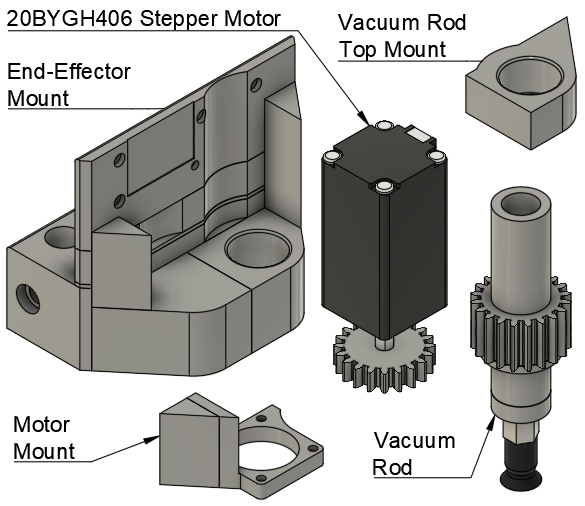
\includegraphics[width=0.6\linewidth]{figures/202107/end-effector-disassembled.png}
 \caption{Disassembled end-effector mount assembly.}
 \label{fig:end-effector-disassembled}
\end{figure}

\begin{figure}[H]
	\centering
	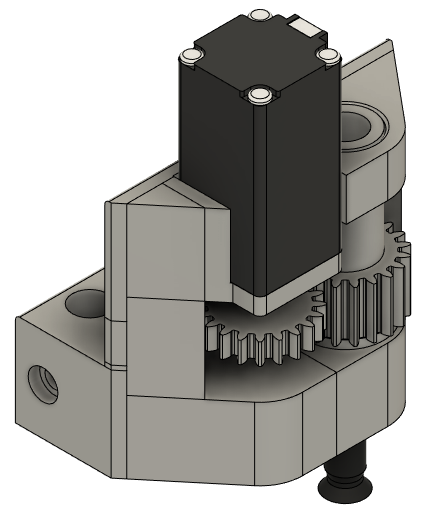
\includegraphics[width=0.3\linewidth]{figures/202107/end-effector-assembled.png}
	\caption{Assembled end-effector mount assembly.}
	\label{fig:end-effector-assembled}
\end{figure}

\subsection{Z-Axis Assembly}

For the purposes of this project, the z-axis assembly is defined as the collection of mechanical components that move linearly along the z-axis when the z-axis drive mechanism is activated. In the case of this project, the z-axis drive mechanism is included in the z-axis assembly. There are many different approaches to the z-axis mechanism. One of the most common approaches which is often used in \ac{CNC} applications involves the use of a linear guide which is fixed with respect to the motion of the z-axis assembly. The z-axis drive mechanism is also fixed with regards to the z-axis assembly. In other words, when the z-axis drive is activated, the z-axis assembly moves relative to the linear guides and the linear drive. The advantage of this approach is that the moving mass of the z-axis assembly is minimised as the linear guides and the z-axis drive mechanism are fixed relative to the motion. The linear bearings form part of the z-axis assembly in this case. The disadvantage of this approach is that a connecting component is required to connect the end-effector to the point at which the linear bearings connect to the linear guides. As such, the greater the range of motion along the z-axis that is required, the longer this connecting element has to be. This introduces a potential area of play as the connecting component is prone to a greater degree of flex the greater its length is. Therefore, this approach is only suited to tasks in which the range of motion along the z-axis is minimal.

Another variation of this approach is to include the linear guides as well as the z-axis drive as part of the z-axis assembly that moves along the z-axis. In this arrangement, the linear bearings are fixed with regards to the motion of the z-axis assembly. The disadvantage of this approach is that there is greater moving mass along the z-axis but this is allows a greater range of motion to be achieved along the z-axis. Since the nature of this project requires a reasonably large range of motion along the z-axis, this latter approach was selected.

With the approach including both the z-axis drive mechanism as well as the linear guides as part of the z-axis assembly, there are two primary design decisions. These are with regards to the selection of the linear guide components as well as the selection of the linear drive mechanism. The most popular drive mechanisms are the lead screw drive solution and the timing belt based drive mechanism. Timing belts are beneficial when the load needs to be moved over a relatively large distance at a relatively high speed. However, they generally require larger motors with more torque. Therefore, they are suited to motion along directions where they are not working against gravity. Lead screw drives, on the other hand, generally require small motors with less torque to drive the same load and are suited to moving loads slowly and accurately over small distances. Since the z-axis motor forms part of the moving z-axis assembly in the design approach discussed above, a smaller motor is preferable to reduce the moving mass of the assembly. Secondly, the range of motion along the z-axis is relatively small compared to the range of motion required along the x and y axes. Therefore a lead screw drive approach was selected for the z-axis assembly.

There are two popular linear guide mechanisms with regards to motion along the z-axis. The first is the linear rail guide which has excellent characteristics when it comes to resisting forces and torque in any other direction than its line of travel. Unfortunately, these preferable characteristics come at a cost. The linear rails in themselves are not completely stiff and need to be mounted to a supporting structure such as an aluminium v-slot extrusion which would increase the moving mass of the z-axis assembly to an unreasonable level. Secondly, the financial cost of the linear rails per relatively high. Therefore, linear rails were not selected for linear motion along the z-axis. Rather the alternative linear guide mechanism, namely linear rods, was selected instead. Specifically, 8mm diameter chromed steel linear rods were selected since they are one of smallest linear rod diameters available and the vertical nature of the z-axis assembly does not exert much torque on the linear rails.

\FigRef{fig:end-effector-disassembled} shows that the end-effector mount already incorporates mounting points for the linear rods. A custom component needed to be designed to complete the z-axis assembly and needed to perform the following functions:

\begin{compactitem}
	\item It should provide a mounting location for the 35BYGH312P1 stepper motor in an orientation with the drive shaft at the bottom aligned with the z-axis.
	\item It should provide mounting points for the 8mm diameter linear chromed steel rods.
	\item It should provide a mounting point for the first line of the drag chain that will be used to route the cables for the 20BYGH406 stepper motor, the 35BYGH312P1 stepper motor and finally the vacuum tubing coming from the vacuum rod.
\end{compactitem}

\FigRef{fig:z-axis-motor-mount} shows the component that was designed in order to meet these requirements. The component was designed in a such a manner that it is amenable to being manufactured using the process of \ac{FDM} 3D printing with the use of supports for the overhang used to mount the drag chain link.

\begin{figure}[H]
	\centering
	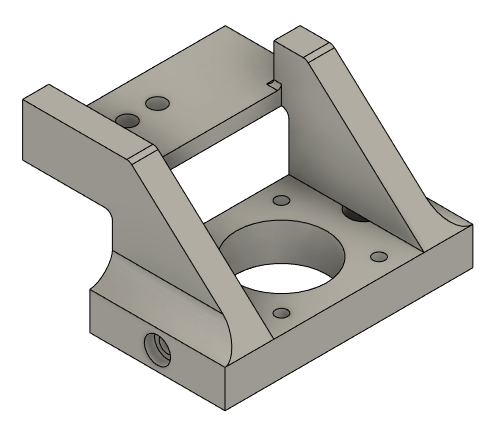
\includegraphics[width=0.4\linewidth]{figures/202107/z-axis-motor-mount.png}
	\caption{Z-axis motor mount.}
	\label{fig:z-axis-motor-mount}
\end{figure}

The components that the z-axis assembly comprises of are summarised in the list below:

\begin{compactitem}
	\item End-effector mount assembly
	\item Z-axis motor mount
	\item 8mm diameter, 8mm pitch lead screw of length 168mm
	\item 8mm diameter to 5mm diameter rigid coupling to connect the lead screw to the shaft of the stepper motor
	\item 35BYGH312P1 stepper motor
	\item, 2x 8mm diameter linear chromed steel rods of length 195mm
\end{compactitem}

\FigRef{fig:z-axis-assembly} shows how all of these components are integrated to form the final z-axis assembly.

\begin{figure}[H]
	\centering
	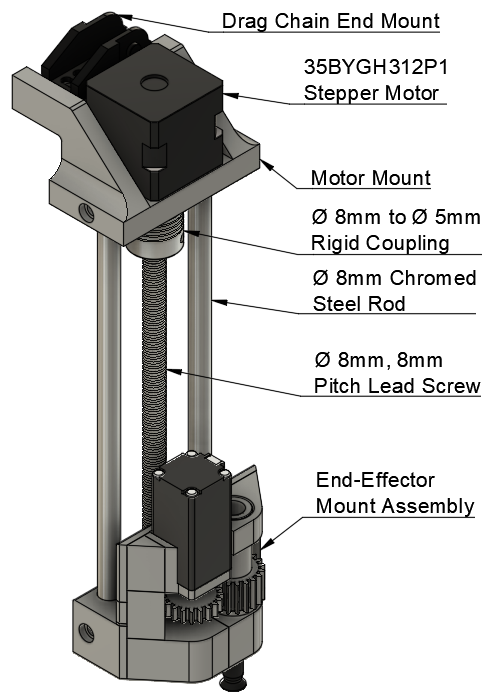
\includegraphics[width=0.6\linewidth]{figures/202107/z-axis-assembly.png}
	\caption{Z-axis assembly.}
	\label{fig:z-axis-assembly}
\end{figure}

\pendsign


\section[2021/07/29]{Friday, 29 July 2021}

\subsection{Stepper Motor Driver}

The DRV8825 stepper motor driver was selected to control the stepper motors used in the project primarily due to its availability in the ISG hardware store. The following important features are noted from the device's datasheet:

\begin{compactitem}
	\item 1/32 Microstepping
	\item 8.2 V to 45 V Operating Supply Voltage Range
	\item Low Current Sleep Mode
	\item Fault Condition Indication Pin
\end{compactitem}

The DIR input pin level is used to select the direction of rotation of the stepper motor while a rising edge on the STEP input pin of the driver causes the microstepping indexer to advance one step. The MODEX input pins are used to set the microstepping of the driver. The board on which the DRV8825 is mounted sets some of the pins to fixed configurations which cannot be altered through the board interface pins as shown in \FigRef{fig:drv8825-schematic}. One such pin is the DECAY input pin which selects the decay mode of the driver to mixed decay by leaving the pin open.

\begin{figure}[H]
	\centering
	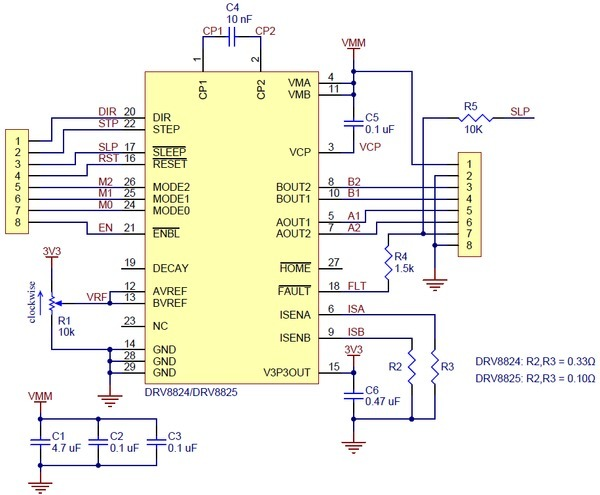
\includegraphics[width=0.9\linewidth]{figures/202107/drv8825-schematic.jpg}
	\caption{DRV8825 schematic}
	\label{fig:drv8825-schematic}
\end{figure}

The timing requirements for the stepping command pulses on the STEP pin are shown in \FigRef{fig:drv8825-timing-requirements}.

\begin{figure}[H]
	\centering
	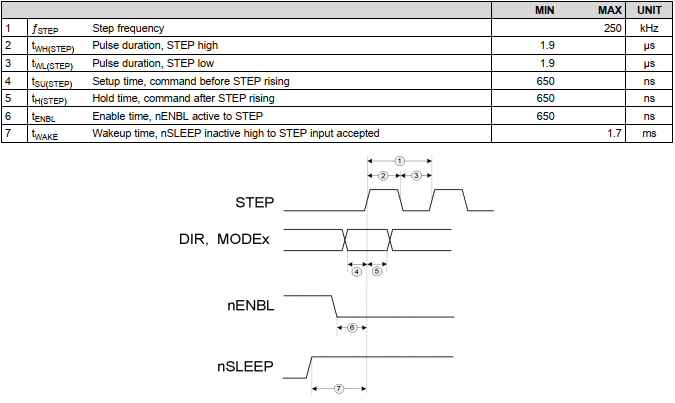
\includegraphics[width=1\linewidth]{figures/202107/drv8825-timing-requirements.png}
	\caption{DRV8825 timing requirements}
	\label{fig:drv8825-timing-requirements}
\end{figure}

\pendsign

\section[2021/07/30]{Friday, 30 July 2021}

\subsection{Microcontroller Selection}

The project requires an embedded platform to control the robotic subsystem and communicate with the PC. A microcontroller needs to be selected to control the robotic subsystem stepper motors by means of the DRV8825 stepper motor drivers as well as the servo that controls the vacuum subsystem. Furthermore, the microcontroller needs to be capable of monitoring the pressure sensor reading of the vacuum subsystem as well as the mechanical limit switches for the three Cartesian axes. The specific microcontroller pin requirements to control and monitor each individual stepper motor DRV8825 board are shown below:

\begin{compactitem}
	\item 2 x digital output pins to control the DRV8825 STEP and DIR (direction)  input pins.
	\item 1 x digital input pin to monitor the DRV8825 FAULT output pin.
\end{compactitem}

Since 4 DRV8825 stepper motor drivers are to be used, this requires 8 digital output pins and 4 digital input pins. In Furthermore, the following pins will be used to control all the stepper motor drivers with a single signal:

\begin{compactitem}
	\item 6 x digital output pins to control the DRV8825 EN (enable), RST (reset), SLEEP and M[0:2] (microstepping) input pins with a shared signal for all drivers.
\end{compactitem}

A single digital output pin is also required to control the vacuum system servo motor. The microcontroller needs to have sufficient computational power to simultaneously control the 4 stepper motors according to various acceleration profiles, control the vacuum subsystem servo motor, monitor the vacuum subsystem pressure and communicate with the PC. The stepper motor control and acceleration computations are expected to use the most computation time. Furthermore, the use of microstepping to achieve smooth stepper motor motion also increases the computational load as more step pulses need to be sent to the stepper motor drivers per unit time. An 8-bit microcontroller could possibly achieve this performance with highly optimised code. However, the rules of EPR 402 forbids the use of an 8-bit microcontroller. 32-bit microcontrollers offer greater computational power which facilitate greater leeway in the stepper motor control computations. Furthermore, the current trend in industry, especially in the 3D printing space, is towards 32-bit controller boards. For these reasons, it was decided to use a 32-bit microcontroller as the basis for the embedded platform.

The general design of 3D printers is similar to the design of the robotic subsystem required in this project in terms of the size of the robotic subsystem, the Cartesian nature of the robot and the number of stepper motors that require control. Therefore, the control board required to be developed for this project will bear resemblance to many existing 3D printer control boards. For this reason, the common microcontrollers used on these control boards were researched and listed below as a starting point for selection:

\begin{compactitem}
	\item The LPC1769 microcontroller is used on the Smoothieboard v1 and SKR 1.4 Turbo boards.
	\item The STM32F103RCT6 microcontroller is used on the SKR Mini E3 and Creality Ender-3 V2 board.
	\item The Atmel SAM4E8E microcontroller is used on the Duet 2 Wifi board.
	\item The LPC1768 is used on the MKS SBASE V1.3 (note this board also makes use of the DRV8825 stepper motor drivers) and Re-ARM boards.
	\item The SAM3X8E microcontroller is used on the Archim2 board.
\end{compactitem}

\pendsign